% !TEX program = pdflatex
%%%%%%%%%%%%%%%%%%%%%%%%%%%%%%%%%%%%%%%%%
% Structured General Purpose Assignment
% LaTeX Template
%
% This template has been downloaded from:
% http://www.latextemplates.com
%
% Original author:
% Ted Pavlic (http://www.tedpavlic.com)
%
% Note:
% The \lipsum[#] commands throughout this template generate dummy text
% to fill the template out. These commands should all be removed when
% writing assignment content.
%
%%%%%%%%%%%%%%%%%%%%%%%%%%%%%%%%%%%%%%%%%

%----------------------------------------------------------------------------------------
%	PACKAGES AND OTHER DOCUMENT CONFIGURATIONS
%----------------------------------------------------------------------------------------

\documentclass{article}

\usepackage{fancyhdr} % Required for custom headers
\usepackage{lastpage} % Required to determine the last page for the footer
\usepackage{extramarks} % Required for headers and footers
\usepackage{graphicx} % Required to insert images
\usepackage{subcaption}
\usepackage{lipsum} % Used for inserting dummy 'Lorem ipsum' text into the template

\usepackage[utf8]{inputenc}
\usepackage[ngerman,english]{babel}
\usepackage[T1]{fontenc}
\usepackage{breakurl}
\usepackage[hyphens]{url}
\usepackage{color}
\usepackage{float}
\usepackage{hyperref}
\usepackage{tabularx}
\usepackage{enumitem}
\usepackage{color, colortbl}
\usepackage[super]{nth}
\usepackage{wrapfig}
\usepackage{amsmath}

\usepackage[
	backend=biber,
	style=numeric-comp,
	natbib=true,
	url=false,
	doi=false,
	eprint=false,
	sorting=none,
	isbn=false]
	{biblatex}

\bibliography{references}

\addto\captionsenglish{
  \renewcommand{\contentsname}%
    {Table of Contents}%
}

% Margins
\topmargin=-0.45in
\evensidemargin=0in
\oddsidemargin=0in
\textwidth=6.5in
\textheight=9.0in
\headsep=0.25in

\linespread{1.1} % Line spacing
% Set up the header and footer
\pagestyle{fancy}
\lhead{} % Top left header
\chead{} % Top center header
\rhead{\firstxmark} % Top right header
\lfoot{\lastxmark} % Bottom left footer
\cfoot{} % Bottom center footer
\rfoot{Page\ \thepage\ of\ \pageref{LastPage}} % Bottom right footer
\renewcommand\headrulewidth{0.4pt} % Size of the header rule
\renewcommand\footrulewidth{0.4pt} % Size of the footer rule

\setlength\parindent{0pt} % Removes all indentation from paragraphs


\begin{document}
\setcounter{tocdepth}{2} % No subsubsections


%----------------------------------------------------------------------------------------
% TITLE PAGE
%----------------------------------------------------------------------------------------
\pagenumbering{gobble}
% \maketitle
\begin{titlepage}
  \centering
\includegraphics[width=5cm]{pictures/tumlogo}

  \vspace{2.5cm}
  \Huge{Trainingswissenschaften} \\
  \vspace{0.1in}\huge{Zusammenfassung}\\

  \Large
  \vspace{1.5cm}
  \begin{tabularx}{9cm}{r l}
    Author: & Thomas Pettinger\\
            & Nils Kunze\\
  \end{tabularx}

  \vfill
  \textbf{2016-07-20} \\
  \vspace{0.3in}\normalsize{Trainingswissenschaften}\\
  \vspace{0.03in}\normalsize{\textsc{Technische Universität München}}\\
  \vspace{1cm}

\end{titlepage}
%----------------------------------------------------------------------------------------


\newpage
\thispagestyle{empty}
\tableofcontents

\newpage
\pagenumbering{arabic}

%!TEX root = ../report.tex

\section{Einführung}

\subsection{Trainingswissenschaft}
\begin{itemize}

\item Leistungsfähigkeit: zeitlich überdauernde Eigenschaften eines Individuums
  \begin{itemize}
  \item Konditionelle Komponenten: Ausdauer, Kraft, Schnelligkeit, Beweglichkeit
  \item Informationelle Komponenten: Technik, Taktik
  \item Determinanten: Einzelfaktoren, die die Ausprägung einer (Teil-) Komponente bestimmen
  \end{itemize}
\item Realisation: Aktion zur Bewältigung einer Aufgabe im Sport
\item Training: Maßnahmen zur Steuerung der Leistungsfähigkeit
  \begin{itemize}
    
  \item Training ist die planmäßige und systematische Realisation von Maßnahmen (Trainingsinhalte und Trainingsmethoden) zur nachhaltigen Erreichung von Zielen (Trainingsziele)
im und durch Sport.
  \item Beanspruchung -> Beanspruchungsfolgen -> Adaption \item Unterscheidung zwischen konditionell und informationell
  \item Belastung: objektiv von Außen auf den Organismus wirkende Faktoren
  \item Belastungsnormative: Größen zur Beschreibung des Belastungsreizes (Intensität, Dauer, Umfang,\ldots)
  \item Beanspruchung: individuelle Reaktion des Organismus auf eine Belastung (z.B. gemessen über Herzfrequenz)
  \item Trainingsziele: Ausgewählte Komponenten der Leistungsfähigkeit
  \item Trainingsmethoden: Kombination von Belastungsnormativen zum Ansprechen der Determinanten
  \item Trainingsinhalte: Übungsgut zur Implementierung der Methodik
  \item Der Anwendungskontext von Training, beeinflusst die Ziele und damit die Inhalte und Methoden
  \end{itemize}
\item Leistung: Relativierung von Aktion und -ergebnis (bzw.\ im Wettkampf) an einer Norm
  \begin{itemize}
  \item Leistungsdiagnostik
    \begin{enumerate}
      \item Beschreibung der Realisation
      \item Bewertung der Realisation vor dem Hintergrund einer Norm
      \item Rückschluss auf die Leistungsfähigkeit
      \item Ableitung von Trainingszielen
    \end{enumerate}
  \end{itemize}
\end{itemize}

\newpage
%!TEX root = ../report.tex

\section{Ausdauer}
Definition: Ermüdungswiderstandsfähigkeit (konditionell und informationell) und Regenerationsfähigkeit

\subsection{Systematik}
\subsubsection{Belastungsdauer}
\begin{itemize}
  \item Kurzzeitausdauer (<35s)
  \item Mittelzeit-Ausdauer(35s - 8min)
  \item Langzeitausdauer (> 8min): LZA I: 8-30min, LZA II: 30min - 3h, LZA III: 3-9h, LZA IV: >9h
\end{itemize}

\subsubsection{Allgemeine vs spezielle Ausdauer}
\begin{itemize}
  \item Allgemeine Ausdauer: Grundlage für Regeneration, Training und Erholung und Voraussetzung für spezielles Training
  \item Spezielle Ausdauer: Wettkampfspezifische Ausdauer-Anforderungen (wichtiger für sportlichen Erfolg)
\end{itemize}

\paragraph{KsA: Koeffizient der speziellen Ausdauer}
= durchschnittliche 100m-Zeit obere Nachbarstrecke / durchschnittliche 100m-Zeit untere Nachbarstrecke

\subsection{Energiebereitstellung}
\paragraph{Mechanismen}
\begin{itemize}
  \item Systematik: Je nach Dauer und Intensität der Belastung wird Energie aus verschiedenen Substanzen gewonnen.
  \item Energiegewinnung aus Substrat:
    \begin{itemize}
      \item Energiefluss: Rate, mit der Energie zur Verfügung gestellt werden kann.
      \item Kapazität: Energievorrat
    \end{itemize}
  \item Problem: Maximale Energie nur kurzfristig verfügbar\\
    Dauerleistungsgrenze: ca 40\%
  \item Energiearten
    \begin{itemize}
      \item alaktazid (Cache (high transfer, low capacity))
      \item laktazid (Memory)
      \item aerob (Drive)
    \end{itemize}
\end{itemize}

\subsection{Determinaten der Ausdauer}
\begin{centering}
\begin{tabular}{m{0.2\textwidth} | m{0.3\textwidth} | m{0.3\textwidth}}
                          & Intensiv                                                         & Extensiv \\ \hline
     Energiespeicher      & Phosphat                                                         & Glykogen \\ \hline
     Enzymaktivityät      & Phosphatstoffwechsel Laktatabbau und -toleranz                   & Kohlenhydrat- und Fettstoffwechsel \\ \hline
     Muskulatur           & vortriebrelevante Muskulatur                                     & Haltearbeit verrichtete Muskulatur \\ \hline
     Sauerstoffversorgung & \multicolumn{2}{c}{Schlagvolumen, Kapillarisierung der Arbeitsmuskulatur, Blutmenge} \\ \hline
     Qualität der Technik & \multicolumn{2}{c}{Bewegungsökonomie} \\ \hline
     Psychische Eigensch. & \multicolumn{2}{c}{Durchhaltevermögen, ``Stehvermögen'', ``mentale Härte''} \\
\end{tabular}
\end{centering}

\subsection{Herz-Kreislauf}
\begin{itemize}
  \item Maximale Sauerstoffaufnahme - Normale Werte: 38-42 ml O2/(min x kg) (Frauen) und 44-50 ml O2/(min x kg) \\
    Spitzensportler: ca doppelte Werte
  \item Herzminutenvolumen (abhängig von Herzvolumen und Belastungsherzfrequenz)
    \begin{itemize}
      \item untrainiert: 20 l/min
      \item trainiert: 40 l/min
    \end{itemize}
  \item Blut (abhängig von Blutmenge und Sauerstoffbindungsfähigkeit)
\end{itemize}

\subsection{Methoden nach Trainingsbereichen}
\begin{centering}
\begin{tabular}{m{0.25\textwidth} | m{0.5\textwidth} | m{0.25\textwidth}}
   Trainingsbereich              & Primäres Ziel                                                                   & Methode \\ \hline
   Regeneration                  & Regenerationsbeschleunigung                                                     & Extensive Dauermethode \\ \hline
   Grundlagenausdauer 1          & Ausdauerfähigkeit niedriger Intensitätsbereich                                  & Intensive Dauermethode \\ \hline
   Grundlagenausdauer 2          & Ausdauerfähigkeit hoher Intensitätsbereich und physiol. Kapazitätserweiterungen & Intervallmethoden \\ \hline
   Wettkampfspezifische \newline Ausdauer & Ausdauerfähigkeit im Wettkampfbereich                                           & Wettkampfmethode \\
\end{tabular}
\end{centering}

\subsection{Belastungsmotive und Ausdauertraining}
\begin{itemize}
  \item Intensität: Stärke eines Einzelreizes
  \item Dauer: Wirkungsdauer eines Einzelreizes
  \item Umfang: Dauer \& Zahl der Reize/Trainingseinheit
  \item Dichte: Zeitliches Verhältnis zwischen Belastungs- und Erholungsphasen
  \item Häufigkeit: Zahl der Trainingseinheiten pro Trainingszeitraum
\end{itemize}

\subsection{Methoden im Überblick}
\begin{itemize}
  \item Dauermethode: Ununterbrochene Dauerbelastung mit geringer intensität und keinen Pausen
  \begin{figure}[H]
          \centering
          \begin{subfigure}[b]{0.4\textwidth}
            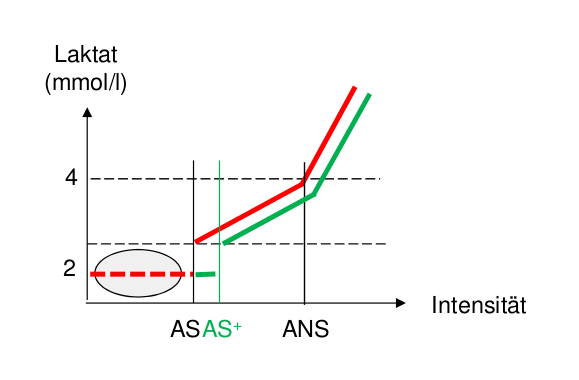
\includegraphics[width=\textwidth]{pictures/dauertraining_extensiv.png}
            \caption{Dauertraining extensiv}
          \end{subfigure}
          \begin{subfigure}[b]{0.4\textwidth}
            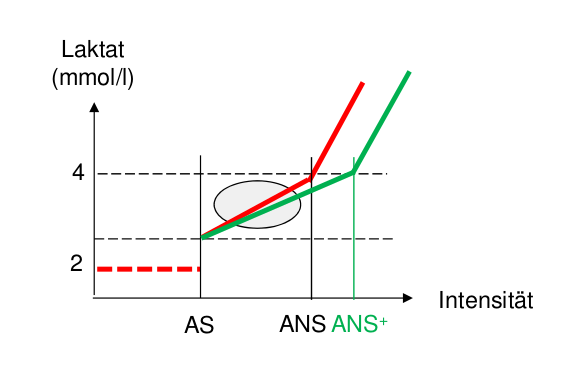
\includegraphics[width=\textwidth]{pictures/dauertraining_intensiv.png}
            \caption{Dauertraining intensiv}
          \end{subfigure}
        \end{figure}
    \begin{itemize}
      \item Extensiv: Intensität unterhalb der AS (?) \& Dauer von 20-60min oder mehr.\\
        Intension: Rechtsverschiebung der AS, Hoher Energieverbrauch, Regeneration, Gewöhnung an Belastungsmonotonie \\
      \item Intensiv: Intensität knapp unterhalb der ANS, Dauer \& Intensität hoch ($\leq$ ED)\\
        Intention: Rechtsverschiebung der ANS, Verbesserung des Glykose- und Laktatabbaus, Laktattoleranz (``MENTALE HÄRTE BITCH'')
    \end{itemize}
  \item Intervallmethoden: Intensität wechselnd über und unter dem ANS, durch Erholungspausen höhere Intensitäten als bei Dauermethoden mgl \\
    Intention: Verbesserung der Leistungsfähigkeit oberhalb der ANS, Phosphatstoffwechsel, hyperthrophie Herzmuskel (Belastungsphase), Erhöhung des Schlagvolumens
    \begin{figure}[H]
      \centering
      \begin{subfigure}[b]{.4\textwidth}
          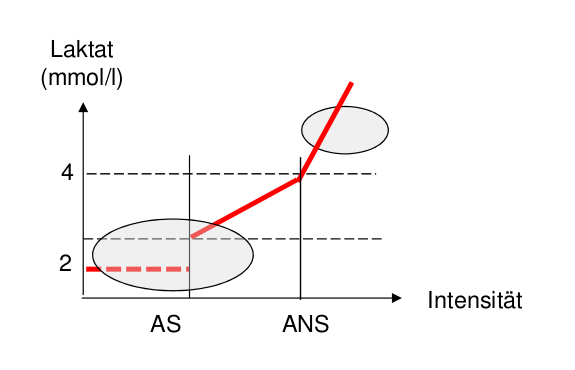
\includegraphics[width=\textwidth]{pictures/intervalltraining.png}
          \caption{Intervallmethoden}
      \end{subfigure}
      \begin{subfigure}[b]{.4\textwidth}
          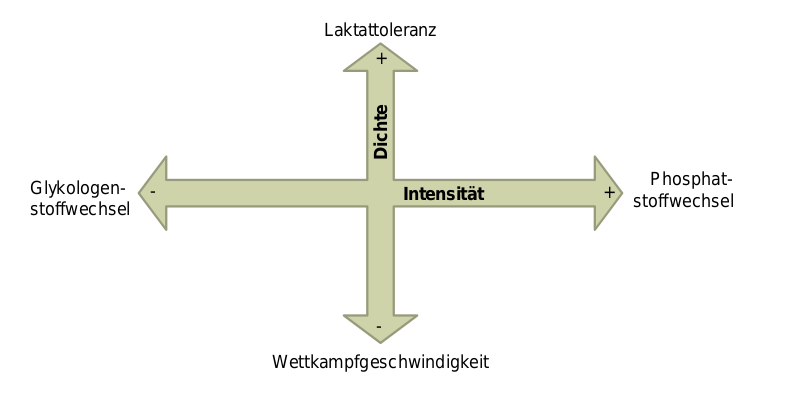
\includegraphics[width=\textwidth]{pictures/akzentuierung_der_trainingswirkung.png}
          \caption{Akzentuierung der Trainingswirkung}
      \end{subfigure}
    \end{figure}

\item Wiederholungsmethode: nahe maximale Intensität, ca. Wettkampfdauer, fast vollständige Pause\\
    Intention: Zusammenspiel aller Energiebereitstellungssysteme, alle physiologischen Prozesse
\item Wettkampfmehode: max. Intensität, mind. Wettkampfdauer, eine vollständige Pause \\
    Intention: Disziplinspezifische Belastungen, Validierung von Taktik, Trainieren der Superkompensation (d. Ausschöpfen von Reserven)\\
    Die Intensität wird beispielsweise durch Laufbandtests festgestellt, bei denen die Herzfrequenz bei erreichen der AS/ANS gemessen wird
\end{itemize}

\subsection{Trainingsinhalte}
Je nach Sportart und Leistungsziel werden andere Trainingsschwerpunkte gesetzt.
\begin{figure}[H]
    \centering
    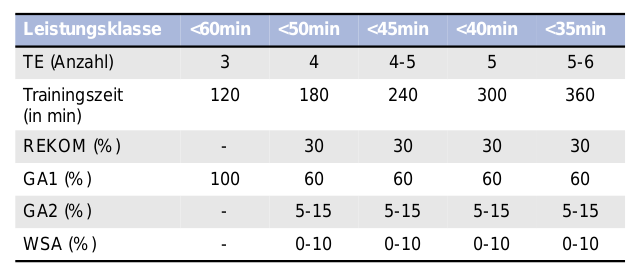
\includegraphics[width=.5\textwidth]{pictures/trainingsbeispiel_tempolauf.png}
    \caption{Trainingsbeispiel für einen Tempolauf über 10km}
\end{figure}

\subsection{Anwendung}
\begin{itemize}
    \item Leistungssport: (Ausdauer als Hauptanteil) REKOM, GA1, GA2, WSA
    \item Leistungssport (Ausdauer nicht Hauptanteil): REKOM (20min), GA1 (30-45min)
    \item Gesundheitssport: GA1 (min: 10-15min, opt: 30-45min)
\end{itemize}

Wirkungen auf die Gesundheit:
\begin{itemize}
    \item Geringere Belastung des Herzes im Alltag
    \item Höhere Resistenz für Infektion, Kälte \& Stress
    \item Positive Wirkung bei Depressionen
    \item Verbesserung der Gedächtnisleistung
    \item Erhöhter Kalorienumsatz
    \item Regulierung des Blutzucker- und Cholesterinspiegels
\end{itemize}
HIIT (High-intensity interval training) wird im Freizeitsport als unkritisch eingestuft.
Mit HIIT können kürzere Trainingszeiten für gleiche Effekte erzielt werden.

\subsection{Medizinische Empfehlung}
Sport wird ab einem Übergewicht von 20\% medizinisch empfohlen (Idealgewicht Körpergröße in cm - 100).
Das Training sollte langsam beginnen (optimal 70\% der maximalen Herzfrequenz), jedoch 10 Minuten 2-3 mal die Woche.
Bei Verbesserung der Leistung erst Häufigkeit und Belastungsumfang (jedoch nicht gleichzeitig), dann erst Intensität.

\subsection{Diagnostik}
\paragraph{Stufentest}
Der Stufentest ist ein Test für die aeroben Kapazität.
Ein Laufband wird benutzt bei dem alle 3 Minuten die Stufe erhöht wird (Anfang 60-100W, Stufe 20W).
Der Test wird abgebrochen wenn die Testperson subjektiv erschöpft ist oder eine festgelegte Geschwindigkeit erreicht wurde.
Mann misst dabei die AS und ANS mittels der Laktatkonzentration und die Geschwindikeit beim Abbruch.
\paragraph{Cooper-Test}
Der Cooper-Test testet die Ausdauerfähigkeiten einer Person.
Der Test besteht aus einem 12 Minuten Lauf bei dem die zurückgelegte Strecke gemessen wird.
Belastet werden dabei vor Allem die aerobe und anaerobe Energiebereitstellung.
\paragraph{Wingate Test}
Der Wingate Test zielt auf die anaeroben Kapazitäten ab.
Er besteht aus einem 30 Sekunden Sprint auf einem Radergometer mit konstant hohem Wiederstand.
Dabei werden die maximale Leistung, relative maximale Leistung, mittlere Leistung und Ermüdungsindex erfasst.
\paragraph{Yo-Yo-Test}
Der Test besteht aus 2x20m Lauf mit steigender Geschwindkeit, anschließend 2x5m Pause.
Der Lauf startet mit 10km/h mit einer Temposteigerung nach 8 Teilläufen um 0.5km/h.
Abgebrochen wird wenn zwei mal in Folge die Zeit nicht eingehalten.

\subsection{Zusammenfassung}
Ausdauertraining kann in jedem Alter ausgeführt werden und hat vielfältige positive Auswirkungen auf die Gesundheit.
Für optimales Training ist eine Kombination aus allgemeinem und spezifischen Methoden notwendig.
Die Grundlagen der Energiebereitstellung können eine Grundlage zum ausarbeiten eines Trainingsplans sein.

\newpage
%!TEX root = ../report.tex

\section{Kraft}

\begin{wrapfigure}{r}{0.5\textwidth}
    \begin{center}
        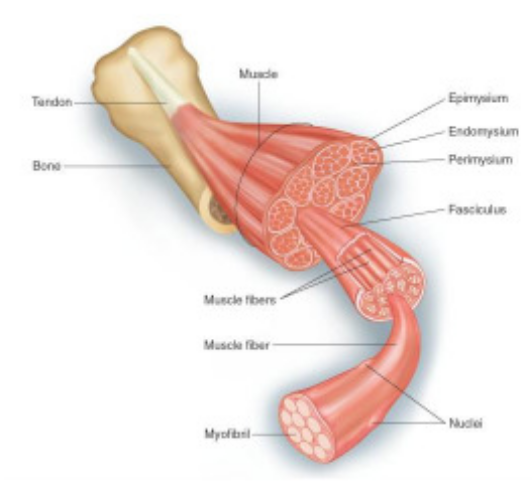
\includegraphics[width=0.48\textwidth]{pictures/muskeln}
    \end{center}
\end{wrapfigure}

Beispiele:
\begin{itemize}
    \item einmalig maximale Kraft (Gewichtheben)
    \item schnell und viel Kraft (Ringen, Hochsprung)
    \item Kraft aufrecht erhalten (Brücke)
\end{itemize}

Anatomische Grundlagen:
\begin{itemize}
    \item grundsätzlich drei Komponenten: Muskel, Sehne, Knochen
    \item Muskel bestehen aus:
    \begin{itemize}
        \item Muskelfaserbündel
        \item Muskelfaser
        \item Myofibrille
        \item Sarkomer
        \item Aktin-Myosin
    \end{itemize}
\end{itemize}

\begin{figure}[h]
\begin{tabular}{|c|c|c|c|}
 \hline
Kontraktionsform & Arbeitsweise & Ansatz / Ursprung & Beispiel Liegestütze \\ \hline \hline
konzentrisch & überwindend & Wird kleiner & Von Boden in Stütz \\ \hline
exzentrisch & nachgebend & Wird größer & Von Stütz auf Boden \\ \hline
isometrisch & haltend & Bleibt gleich & Halten des Stützes \\ \hline
\end{tabular}
\caption{Aktionsformen der Muskeln}
\end{figure}

\subsection{Struktur der Kraft}

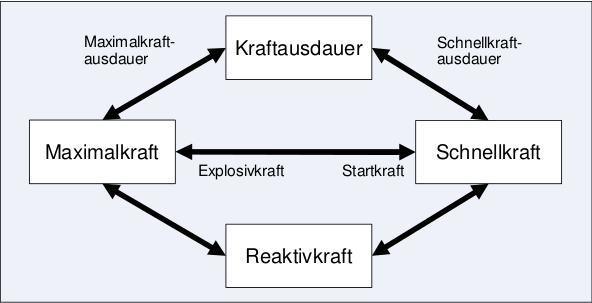
\includegraphics[width=0.9\textwidth]{pictures/kraftstruktur}

\subsection{Determinanten der Kraft}
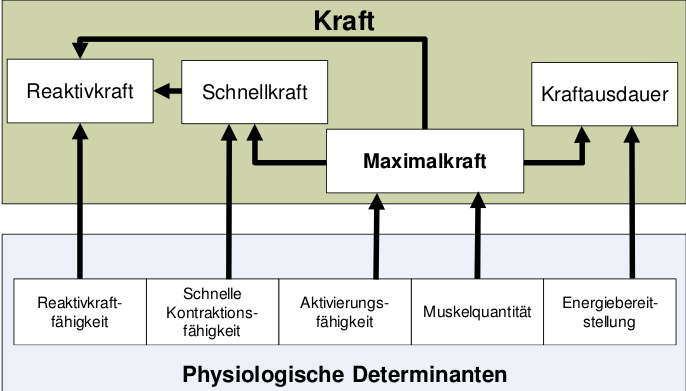
\includegraphics[width=0.9\textwidth]{pictures/kraft_determinanten}

\subsection{Maximalkraft}

[placeholder] % otherwise figure is not at correct position

\begin{wrapfigure}{r}{0.5\textwidth}
    \begin{center}
        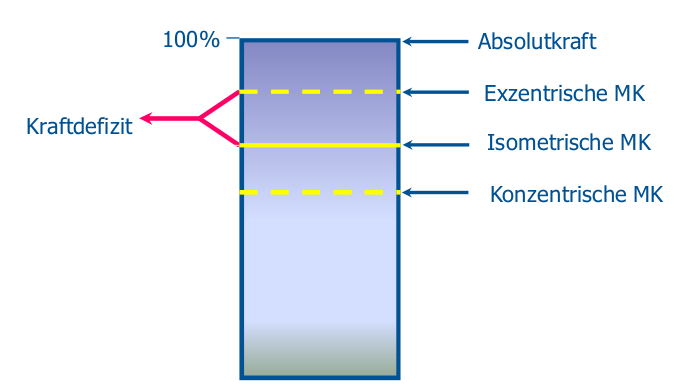
\includegraphics[width=0.48\textwidth]{pictures/maximalkraftvarianten}
    \end{center}
\end{wrapfigure}

[placeholder] % otherwise figure is not at correct position

\begin{itemize}
    \item Definition: Maximalkraft ist die höchstmögliche Kraft, die vom Nerv-Muskel-System willentlich gegen einen Widerstand erzeugt werden kann
    \item 1er-Maximum (1RM = 1 Repetition Maximum) = konzentrische Maximalkraft über volle Bewegungsamplitude
    \item Relativkraft = 1RM / Körpergewicht
    \item bestehend aus:
    \begin{itemize}
        \item Muskelquerschnitt \& Faserzusammensetzung
        \item Willkürliche Aktivierungsfähigkeit
    \end{itemize}
    \item Absolutkraft: Nur durch maximale elektrische Stimulation erreichbare Kraft. Willentlich nicht abrufbar.
    \item Kraftdefizit: $\frac{\text{Exzentrische MK} - \text{Isometrische MK}}{\text{Exzentrische MK}} \cdot 100 \%$
    \item in Praxis: Differenz zwischen isometrischer und exzentrischer MK
    \item Training:
    \begin{itemize}
        \item großes Kraftdefizit: willkürliche Aktivierungsfähigkeit verbessern
        \item kleines Kraftdefizit: Muskelquantität
    \end{itemize}
\end{itemize}

\subsection{Schnellkraft}

[placeholder] % otherwise figure is not at correct position
\begin{wrapfigure}{r}{0.5\textwidth}
  \begin{center}
    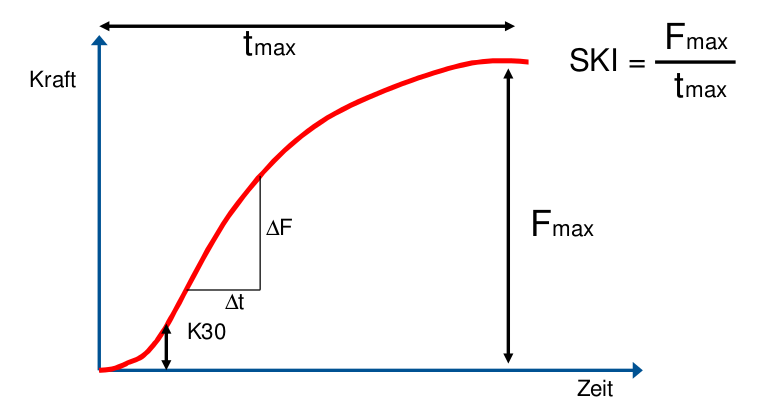
\includegraphics[width=0.48\textwidth]{pictures/kraftanstiegskurve}
  \end{center}
\end{wrapfigure}

\begin{itemize}
    \item Definition: Schnellkraft ist die Fähigkeit, einen möglichst großen Kraftstoß innerhalb einer zur Verfügung stehenden (kurzen) Zeit zu realisieren
    \item Teilaspekte:
    \begin{itemize}
        \item Startkraft (Fähigkeit sehr schnell Kraft zu entfalten, bsp: Boxen?)
        \item Explosivkraft (Fähigkeit großen/schnellen Kraftanstieg zu realisieren, bsp: Würfe, Stöße, Schüsse?)
        \item Dynamisches Kraftmaximum (Fähigkeit MK schnell zu realisieren, bsp: Ringen?)
    \end{itemize}
    \item Struktur der Schnellkraft: Maximalkraft + Schnelle Kontraktionsfähigkeit
    \item Schnelle Kontraktionsfähigkeit hängt ab von Muskelfaserzusammensetzung, Intermuskulärer und Intramuskulärer Koordination
\end{itemize}

\paragraph{Muskelfaserzusammensetzung}
\begin{itemize}
    \item Zusammensetzung genetisch determiniert
    \item Umwandlung praktisch nur Fast Twitch to Slow Twitch durch Ausdauertraining und Querschnittstraining
\end{itemize}
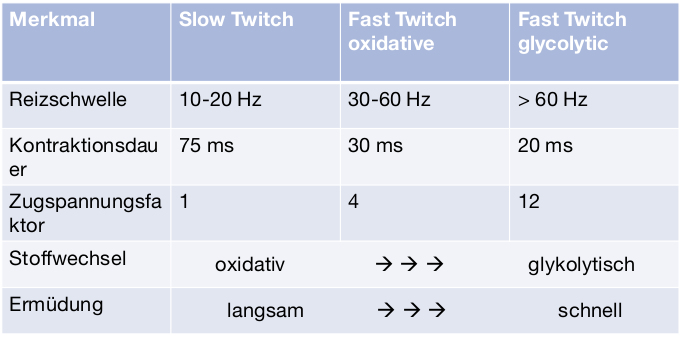
\includegraphics[width=0.9\textwidth]{pictures/muskelfaserzusammensetzung}

\paragraph{Intermuskuläre Koordination}
\begin{itemize}
    \item Zusammenspiel mehrerer Muskeln (Muskelabschnitte)
    \item fertigkeitsspezifisch
    \item kann als Synonym für ``Gute Technik'' betrachtet werden
    \item Grund warum Krafttraining nicht nur auf Stärkung der einzelnen Muskeln ausgelegt sein darf
    \item Beispiele: Fuß-, Knie- und Hüftstrecker bei Strecksprung
\end{itemize}

\paragraph{Intramuskuläre Koordination}
\begin{enumerate}
    \item Sequenzierung: Optimale Reihenfolge der Innervation der Muskelfasern
    \item Frequenzierung: Fähigkeit, den Muskel hochfrequent und nachhaltig zu innervieren
    \begin{itemize}
        \item Je nach Stärke der Erregung über die spinalen Synapsen, feuert ein Motoneuron mit unterschiedlicher Frequenz
        \item  Ab 55 Hz wird Maximale Kraftabgabe möglich
        \item  Bis zu 155 Hz sind möglich und erlauben schnellen Kraftanstieg
    \end{itemize}
    \item Rekrutierung: Fähigkeit, möglichst viele motorische Einheiten zur Kontraktion heranziehen zu können

\newpage
%!TEX root = ../report.tex

\section{Schnelligkeit}
Schnelligkeit ist die Fähigkeit in ermüdungsfreiem Zustand mit möglichst kurzen zeitlichem Abstand auf einen Reiz zu reagieren oder zu agieren.
\begin{figure}[H]
  \centering
  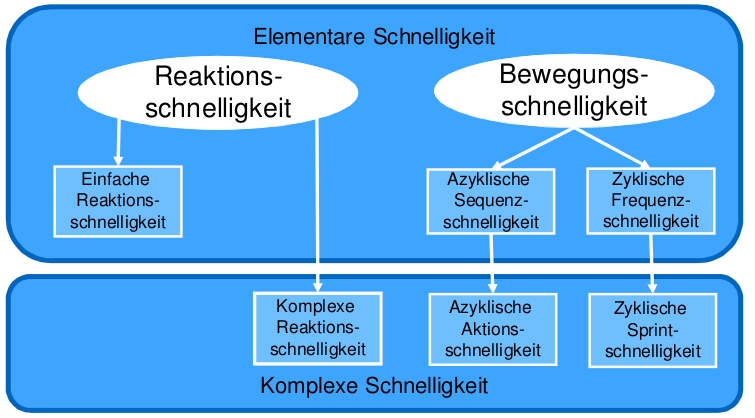
\includegraphics[width=.5\textwidth]{pictures/schnelligkeit_overview.png}
  \caption{Überblick Schnelligkeit}
\end{figure}
\begin{figure}[H]
  \centering
  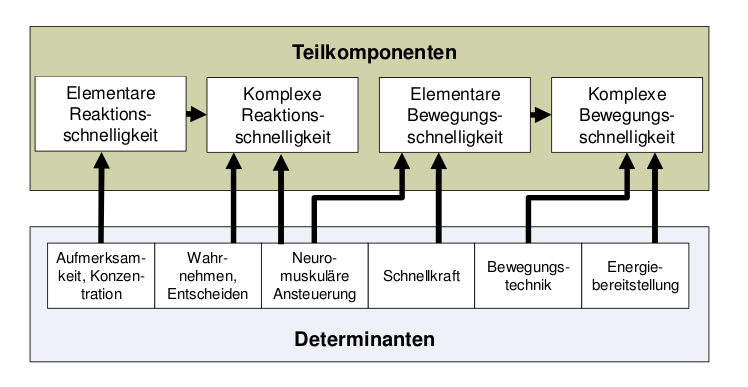
\includegraphics[width=.5\linewidth]{pictures/schnelligkeit_determinanten.png}
  \caption{Determinanten der Schnelligkeit}
\end{figure}

\subsection{Begriffe, Systematik und Determinaten}
\subsubsection{Reaktionsschnelligkeit}
\begin{description}
  \item[Reaktionsfähigkeit] ist die psychophysische Fähigkeit auf Reize schnell zu reagieren.
  \item[Elementare Reaktionsschnelligkeit] Kleinmotorische Bewegungsantworten auf einfache Reize
  \item[Komplexe Reaktionsschnelligkeit] Großmotorische Bewegungsantworten \& komplexe (Wahl-) Reaktionen.
\end{description}

\textbf{Modell der Reaktionsgeschwindigkeit}\\
\begin{figure}[H]
  \centering
  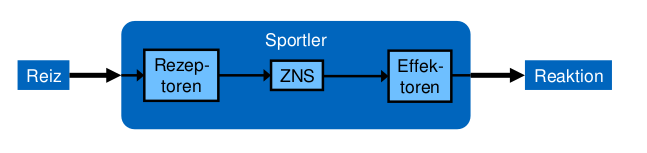
\includegraphics[width=.5\textwidth]{pictures/reaktionsgeschwindigkeit_modell.png}
  \caption{Modell der Reaktionsgeschwindigkeit}
\end{figure}
\begin{description}
    \item[Übertragung bis Rezeptor] hängt vorwiegend von den Eigenschaften des Rezeptors ab (1-20ms).
    \item[Restliche ÜBertragung] wird von den Eigenschaften des Nervensystems beeinflusst (Rezeptor $\rightarrow$ ZNS: 1-100ms, ZNS $\rightarrow$ Effektor: 10-20ms).
    \item[Verarbeitung im ZNS] wird beeinflusst von psychischen Eigenschaften wie Aufmerksamkeit und Wahrnehmung und kann von 70 bis 300ms dauern.
    \item[Verarbeitung in den Effektoren] Abhängig von neuromuskulären Eigenschaften wie Fastetypzusammensetzung oder inter-/intramuskuläre Koordination
\end{description}
Die gesammte Übertragungszeit beträgt in etwa 112 - 510ms.

\subsubsection{Bewegungsschnelligkeit}
Bewegungsschnelligkeit ist die Fähigkeit, Bewegungen in höchster Geschwindigkeit oder kürzester Zeit auszuführen.
\begin{figure}[H]
    \centering
    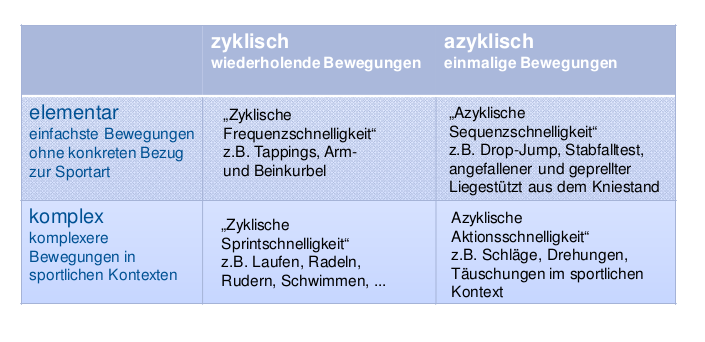
\includegraphics[width=.7\textwidth]{pictures/bewegungsgeschwindigkeit_struktur.png}
    \caption{Struktur der Bewegungsschnelligkeit}
\end{figure}

Die Bewegungsschnelligkeit hängt von drei Bereichen ab:
\begin{description}
    \item[Neuromuskuläres System] Neuronale Steuer- \& Regelprozesse, Reaktionsgeschwindigkeit, inter/intra-muskuläre Koordination,\ldots
    \item[Psychisches System] Konzentration, Wahrnehmung, Motivation, \ldots
    \item[Tendomuskuläres System] Querschnittsfläche FT-Fasern, Stiffness, Viskosität, \ldots
\end{description}

\subsection{Trainingsmethoden}
Schnelligkeit ist schlechter zu trainieren als Ausdauer oder Kraft.\\
Zu trainierende Determinanten sind:
\begin{figure}[H]
    \centering
    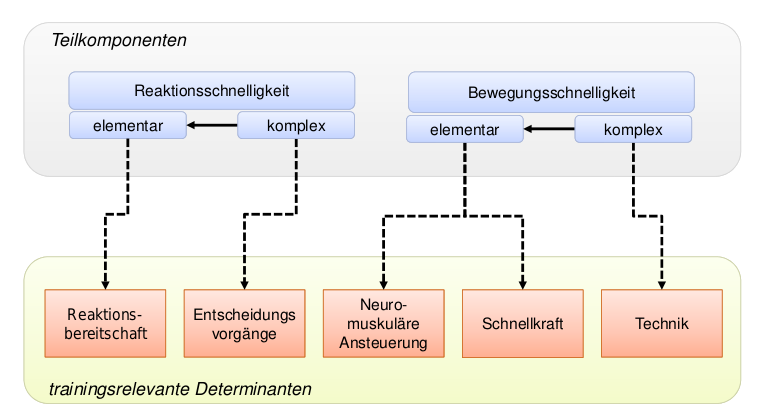
\includegraphics[width=.7\textwidth]{pictures/schnelligkeit_trainierbare_determinanten.png}
    \caption{Trainierbare Determinanten}
\end{figure}

\paragraph{Belastungsnormative}
\begin{description}
    \item[Intensität] Bewegung auf maximaler Geschwindigkeit
    \item[Dauer] 8-10s, Abbruch bei Erschöpfung
    \item[Pause] bis vollständig regeneriert, Schnelligkeitstraining vor anderen
    \item[Durchführung] Mit maximaler Konzentration \& Willen, mit Aufwärmen
\end{description}

\subsubsection{Reaktionsbereitschaft}
Training beinhaltet einfache Reaktionen (Pfiff, (Nacken- :P) Klatschen) auf akustische, visuelle oder taktile Reize.

\subsubsection{Entscheidungsvorgänge}
Eine Wahlreaktion wird vor einer motorischen Reaktion eingefordert.
Auch die richtige Wahrnehmung ist wichtig, Signal wird erschwert zu verstehen (leiser Pfiff = noop, lauter Pfiff = go)

\subsubsection{Neuromuskuläre Ansteuerung}
Grundbewegungen schnell realisieren. Es wird unterschieden zwischen zyklischen (wiederholenden) und azyklischen (einmaligen) Bewegungen.
\paragraph{Geschwindigkeitsbarriere} Häufige Realisation der Maximalgeschwindigkeit führt zu einer Verfestigung der neuromuskulären Ansteuerung (Reizleitungswege, Innervationsmuster).
Gegenmaßnahmen sind nur wenig Wettkampfsimulationen mit Maximalgeschwindigkeit (1/Woche), Variation der Bewegung und Entwicklung der elementaren Fähigkeiten
\paragraph{Erleichterte Bedingungen} Erleichtern der Übungen durch verringern des Wiederstands oder Körpergewichts um Geschwindigkeit zu erhöhen.
Beispiele sind Treppenläufe bergab (zyklisch) oder leichtere Wurfgeräte (azyklisch).
\paragraph{Räumliche Zwänge} Erzwingen einer höheren Frequenz durch Einengungen (z.B. Fesseln).
\paragraph{Mentales Training} Der Carpenter-Effekt (Denken an eine Bewegung bewirkt diese in einem abgeschwächtem Maß) wird dazu genutzt mit Metaphern in der Übungsbeschreibung eine Aktion hervorzurufen (``Springe wie ein Frosch'').
\paragraph{Elektromyostimulation} Elektrische Stimulation auf das Innervationsmuster. Die nicht belegte Hypothese ist dass dadurch eine bessere Rekrutierung motorischer Einheiten erfolgt und das bestehende Innervationsmuster ``überschrieben'' wird.

\subsubsection{Technik}
Technikübungen sind disziplinspezifisch, schnell ausgeführte Bewegungen die meist überbetont werden.
Kombinationen aus einzelnen Aktionen und Übungen sind möglich.

\subsubsection{Schnellkraft}
Eine Erschwerung der Bedingungen (z.B. Laufen mit Zugschlitten) führt zu einem Training für Kraft und Schnelligkeit.
Dadurch ist allerdings die maximale Geschwindigkeit nicht mehr zu erreichen.

\newpage
%!TEX root = ../report.tex

\section{Beweglichkeit}

Definition Beweglichkeit: Beweglichkeit ist die motorische Fähigkeit, Bewegungen willkürlich mit der erforderlichen Schwingungsweite ausführen zu können.

Verwandte Begriffe: \textbf{Gelenkigkeit} = Schwingungsweite von Gelenken, \textbf{Dehnfähigkeit} = Dehnbarkeit von Muskeln und Sehnen

Optimalitätseigenschaft: Stabilität versus Mobilität, Hypo- versus Hypermobilität

\subsection{Systematik und Determinanten}

\subsubsection*{Dimensionen }

\begin{minipage}{0.7\textwidth}
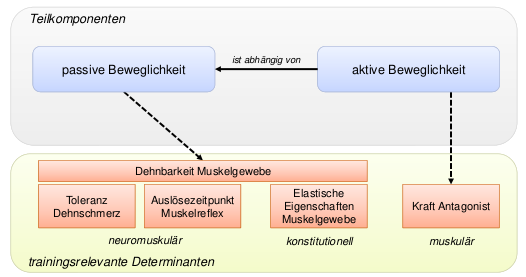
\includegraphics[width=\textwidth]{pictures/beweg_determinanten4}
\end{minipage}
\begin{minipage}{0.3\textwidth}
\begin{itemize}
    \item Passive Beweglichkeit: Beweglichkeit die unter Einwirken einer externen Kraft erreicht wird (z.B. Spagat, Schwerkraft)
    \item Aktive Beweglichkeit: Beweglichkeit, die durch aktive Muskelarbeit erreicht wird (z.B. Armschwung, Schuss, Spagatsprung)
\end{itemize}
\end{minipage}

Methoden im Beweglichkeitstraining:
\begin{itemize}
    \item aktiv: Antagonisten bewirken Dehnung
    \item passiv: Partner, Schwerkraft, andere Muskeln bewirken Dehnung
    \item statisch: langsames Einnehmen der Dehnposition, ohne Auslösung des Muskelreflexes (intensiv)
    \item dynamisch: schnelles, federndes Einnehmen der Dehnposition, mit (unter Inkaufnahme der) Auslösung des Muskelreflexes
\end{itemize}

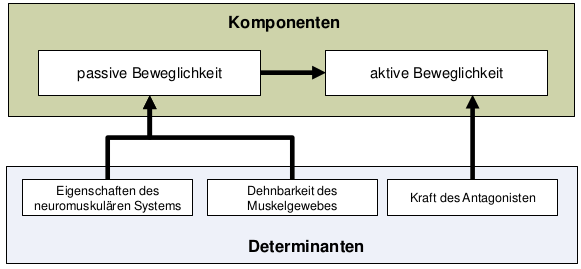
\includegraphics[width=0.9\textwidth]{pictures/beweg_determinanten2}

\subsubsection*{Muskelreflex}

Schnelle Bewegungen lösen den Muskelreflex aus, aber das Auslösen des Muskelreflexes ist kontraproduktiv zur Absicht der Dehnung. Wenn die Dehnung intensiv sein soll, sollte Muskelreflex nicht (nur minimal) ausgelöst werden, d.h. keine schnellen Bewegungen.

Der Muskeltonus ist Ausdruck des systemischen Erregungszustandes. Zu hoch impliziert sanfte Dehnung und Entspannungsübungen, zu niedrig dagegen intensive Dehnung.

Allgemein:
Ein Gelenk besteht aus Muskeln und Sehnen, Knochen, Knorpel und der Gelenkkapsel mit Bändern.
Es gibt verschiedene Rezeptoren:
\begin{itemize}
    \item Ruffini-Körperchen sind Mechanorezeptoren in Kapsel und Haut und reagieren auf Druck und Dehnung. Dabei registrieren sie das Ausmaß und die Geschwindigkeit von Gelenkbewegungen.
    \item Vater-Pacini-Körperchen sind Mechanorezeptoren im Gelenkbindegewebe und registrieren Beschleunigungen.
    \item Golgi-Sehnenorgan sitzt im Übergang zwischen Muskeln und Sehnen und registriert dort die Muskelspannung. Unter Umständen gibt es eine Reflexantwort.
    \item Muskelspindeln sind quergestreifte Muskelfasern, die ebenfalls als Mechanorezeptoren dienen. Sie lösen den Eigenreflex aus und messen das Ausmaß und die Geschwindigkeit einer Muskelbewegung.
\end{itemize}

\subsubsection*{Determinanten}

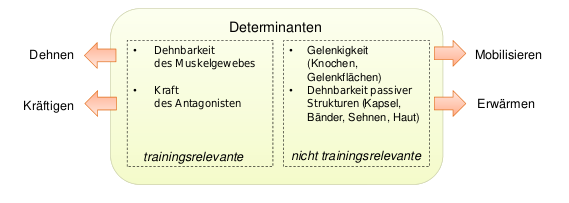
\includegraphics[width=\textwidth]{pictures/beweg_determinanten3}

\begin{minipage}{0.4\textwidth}
Entscheidend sind folgende anatomische Eigenschaften:
\begin{itemize}
    \item Freiheitsgrade und Funktionstüchtigkeit der Gelenke
    \item Bandhafte- und kapsuläre Hemmung
    \item Titinfilamente (hauptsächlich verantwortlich für Widerstand)
    \item Tendo-muskuläre Reflexschaltungen (Hemmungen)
\end{itemize}
\end{minipage}
\begin{minipage}{0.6\textwidth}
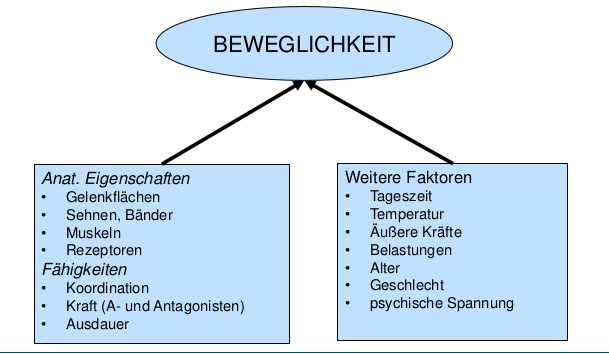
\includegraphics[width=\textwidth]{pictures/beweg_determinanten}
\end{minipage}
Weitere Einflussfaktoren:
\begin{itemize}
    \item Alter: Abnahme der Elastizität (H 2 O-Verlust; Weniger Zellen)
    \item Geschlecht: Einfluss des Östrogens
    \item Ausdauer: Kein Beweglichkeitstraining im Ermüdungszustand
\end{itemize}

\subsection{Bedeutung}

Beweglichkeit kann Bestandteil von Wettkampfleistungen sein (Bsp: bessere Bepunktung von Spagat in der Gymnastik) oder Voraussetzung für Wettkampfleistungen, konditionelle Fähigkeiten oder Teilleistungen sein (Bsp: bessere performance von beweglicheren Fußballspielern).

Als Beweglichkeitsreserve bezeichnet man die Differenz zwischen erforderlichem und maximalem Bewegungsausschlag. Eine große Reserve ist erstrebsam, weil dann nicht bis an die Dehnbarkeitsgrenze belastet werden muss (Ökonomisierung) und die Bewegung unter geringerem Widerstand ablaufen kann. Auch im Fitness- und Gesundheitstraining ist Dehnen zur Vermeidung von Dysbalancen und Verkürzungen relevant.

\subsubsection*{Aufwärmen vs Dehntraining}

Seit Mitte der 90er Jahren ist bekannt, dass intensives statisches Dehnen (Stretching) in der Aufwärmphase genau das Gegenteil von dem, was man sich erhofft, bewirkt.
Statt leistungssteigernd und verletzungsmindern zu wirken, führt es zu geringerer Leistung und einem größerem Verletzungsrisiko. Ausmaß: 4-8\% weniger vertikale Sprungleistung und 5-10\% Reaktivkraftleistungen

Gründe:
\begin{itemize}
    \item Geringere Kraftproduktion Muskel-Sehnen-Komplex (Verlängerung, Belastung der fibrillären Strukturen)
    \item Periphere neuromuskuläre Veränderungen, z.B. Reduktion der
    \item Erregbarkeit der Motoneurone
    \item Zentrale psychophysiologische Desaktivierungsprozesse, Senkung der zentralen Aktivierung
\end{itemize}

Verletzungsprophylaxe: Kräfte bei passiver Dehnung können sehr groß und unphysiologisch werden, zusätzliche steht ein epidemiologischer Nachweis der Verletzungsprophylaxe-Wirkung von intensivem Dehnen noch aus. Muskelkater kann durch (zu) intensives Dehnen verschlimmert bzw. sogar herbeigeführt werden...

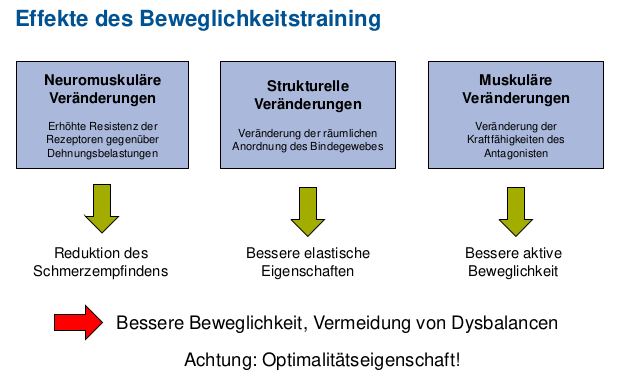
\includegraphics[width=0.9\textwidth]{pictures/beweg_effekte}

\subsection{Diagnostik}

Motorische Beweglichkeits-Tests z.b. mit ablesen auf einer Zentimeterskala und abgleich gegen Normtabelle. Problem von Normwerten: Liefern nur erste Hinweise

Ein anderes klassisches Verfahren zur einfachen Bestimmung von Beweglichkeitseinschränkungen in der Muskulatur  ist der Janda-Test.
Beispiel für den Hüftlendenmuskel: Rückenlage, Oberschenkel beugen und Richtung Brust heranziehen, dabei muss die Lendenwirbelsäule komplett aufliegen.
Anzeichen für Beweglichkeitseinschränkung: der Oberschenkel der Gegenseite geht nach oben.

\subsection{Trainingsmethoden}

\paragraph*{Belastungsnormative}
Problem: Wie wählt man die Intensität? \% des maximalen Bewegungsumfangs? Subjektives Rating über Schmerzskala?
Dauer, Umfang, Dichte, Häufigkeit weniger wichtig, entscheidend ist die Ausführungsart.

Ausführungsarten:
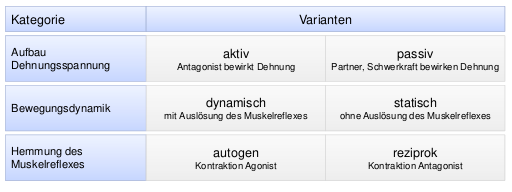
\includegraphics[width=0.9\textwidth]{pictures/beweg_ausfuehrungsarten}

Static Stretching (SS):
\begin{itemize}
    \item Langsame Heranführung an Bewegungsgrenze bewirkt Hemmung des Dehnungsreflexes der Muskeln und Sehnenspindeln
    \item Einnehmen der Dehnposition, so dass deutliche
    Spannung spürbar ist ( = Andehnen).
    \item Wenn das Spannungsgefühl nachlässt, Verstärkung der Dehnung und erneutes Halten ( = Nachdehnen).
    \item Dauer: zwischen 5s und > 60s (je nach Trainingsziel)
\end{itemize}

Contract Relax (CR):
\begin{itemize}
    \item vorgeschaltete Kontraktion des Agonisten führt zur Hemmung des Dehnungsreflexes des Agonist (autogene Hemmung)
    \item Isometrische Kontraktion (submaximal bis maximal) des Agonisten (5s) (C=Contract)
    \item Entspannen des Agonisten (2s) (R=Relax)
    \item Dehnen des Agonisten (aktiv oder passiv)
    \item auch Contract-Hold-Release-Stretch (CHRS) genannt
\end{itemize}

Antagonist Contract (AC):
\begin{itemize}
    \item vorgeschaltete Kontraktion des Antagonisten führt zur Hemmung des Dehnreflexes des Agonisten (reziproke Hemmung)
    \item Anspannen des Antagonisten (5s) (AC)
    \item Dehnen des Agonisten (aktiv oder passiv)
    \item Anspannen und Dehnen, gleichzeitig oder sequenziell
\end{itemize}

Contract Relax – Antagonist Contract (CR-AC):
\begin{itemize}
    \item Ausnutzung beider Effekte
    \item Kontraktion des Agonisten (C)
    \item Entspannung (R)
    \item Dehnen des Agonisten mittels Kontrakation des Antagonisten (AC)
    \item aktiv oder passiv
    \item auch PNF-Dehnen genannt (Propriozeptive neuromuskuläre Fazilitation)
\end{itemize}

Dynamic Stretching (DS):
\begin{itemize}
    \item Nutzung von Schwungkräften
    \item Wiederholtes federn an die Bewegungsgrenze ( = Balistics) oder
    \item langsames „Schieben“ an die Bewegungsgrenze, kurz halten ( = Ballistic \& Hold)
    \item Vorteile: gleichzeitige Kräftigung des Antagonisten und Verbessern der aktiven Beweglichkeit
    \item Nachteile: Dehnreflex, weniger intensive Dehnung möglich
\end{itemize}

\subsection{Trainingsinhalte}

Generelle Hinweise:
\begin{itemize}
    \item Mobilisierung und Aufwärmen vor dem Dehnen
    \item Dehnen möglichst selektiv (eingelenkig)
    \item Beim Dehnen über zwei Gelenke: ein Gelenk fixieren
    \item Keine Dehnung von Muskeln die Haltearbeit leisten müssen
    \item Übungen so wählen, dass Ausweichbewegungen vermieden werde Reihenfolge einhalten
\end{itemize}

Kinder- und Jugendtraining: Eher aktive un dynamische Dehnübungen, Verzicht auf passive und statische Übungen. Außerdem Altergemäß durch Wettbewerbe oder Staffelspiele

\subsection{Anwendung}

Beweglichkeitsmaximierung:
\begin{itemize}
    \item Anwendung: (Hoch-)Leistungssport mit Beweglichkeit als leistungsbegrenzendem Faktor
    \item Methode: CR-AC>AC>CR>SS>DS (nicht nachgewiesen)
    \item Intensität: Maximal (bis an Schmerzgrenze), Einhalten von Belastungsgrenzen!
    \item Dauer: Bindegewebsanpassungen ab ca. 30s (Creeping)
    \item Umfang \& Häufigkeit: eigener Trainingsinhalt , 4-10 Serien, 1-2 Mal täglich, stabile Anpassungen nach ca. 6 Wochen
\end{itemize}

Beweglichkeitserhalt:
\begin{itemize}
    \item Anwendung: sonstiger Leistungssport, Gesundheits- und Freizeitbereich, Leistungsabfall ab 8. Lebensjahr!
    \item Methode: DS (evtl. SS), Dynamisches Dehnen kräftigt zusätzlich!
    \item Intensität: hoch, jedoch nicht bis an die Schmerzgrenze
    \item Dauer: 10-15s in Endposition oder 10 Mal wippen
    \item Umfang \& Häufigkeit: 2-3 Sätze pro Gelenk, 2-3 Mal pro Woche
\end{itemize}

Aufwärmen:
\begin{itemize}
    \item Anwendung: Sportarten in denen Beweglichkeit Vorteile bringt
    \item Pro-Argumente: kurzfristige Gewinne durch Dehnen erzielbar (ca. 8\%)
    \item Effekt der Verletzungsprophylaxe unklar
    \item Contra-Argumente (SS): Fast gleiche Gewinne an Bewegungsreichweite wie beim dynamischen Dehnen, Gefahr von Überlastungen, Durchblutung vermindert und Schnellkraftleistungen sinken kurzzeitig
    \item Methode: DS bevorzugen
    \item Intensität: mittel bis hoch
    \item Dauer: <5s bei maximal- und schnellkraftentwickelnder Muskulatur
    \item 10-15s bei beweglichkeits-relevanter Muskulatur
    \item keine Laktatanhäufung bei aktiven Methoden
    \item Umfang \& Häufigkeit: 1-3 Serien, 15-20 Minuten vor dem Wettkampf
\end{itemize}

Krampfbeseitigung:
\begin{itemize}
    \item Anwendung: Während der Sports, Bei Krämpfen verursacht durch Ermüdung oder mangelnde Versorgung (Blut, Mineralien)
    \item Methode: Vorsichtiges statisches Dehnen des Agonisten (SS) bevorzugen, Kontraktion des Antagonisten
    \item Intensität: gering
\end{itemize}

Cool-Down:
\begin{itemize}
    \item Anwendung: Verbesserung „Körpergefühl“,Verbesserung der Entspannungsfähigkeit,Abbau von Muskelverspannungen,Beschleunigung der Regeneration,Wirkung umstritten!
    \item Methode: SS bevorzugen, alternativ CR
    \item Intensität: eher niedrig bis mittel, sonst "Spülfunktion“ beeinträchtigt
    \item Umfang: 3 Serien nach dem Auslaufen, 5-10s inEndposition halten
\end{itemize}

\subsection{Exkurs: Aufwärmen \& Cool Down}

Aufwärmen:
\begin{itemize}
    \item Varianten:  allgemein vs. speziell, aktiv vs. passiv, physisch vs. mental
    \item Primäreffekte: Anregung Herz-Kreislaufsystem(Kerntemperatur, Atmung, Puls, Blutdruck), Durchblutung Muskultur, Flüssigkeitsregulation Knorpelgewebe
    \item Gewünschte Wirkung: Physische Leistungssteigerung(Sauerstoffversorgung, Erregbarkeit,Muskelviskosität, ...), Verletzungsprophylaxe, Psychische Aspekte
    \item Typisches Aufwärmprogramm (Volleyball): Kreislaufaktivierung, Mobilisation, (Dehnen), Stabilisation, Kurze hochintensive Belastung, Spezielles Aufwärmen mit Ball. Dabei keine Ermüdung induzieren!
\end{itemize}

Mobilisation:
\begin{itemize}
    \item Aufwärmen von Bindegewebe (Bänder, Gelenkkapsel)
    \item Verbesserung der Gleiteigenschaften des Gelenkes
    \item Amplitude nicht ausschöpfen, Funktionsweise des Gelenkes beachten
    \item ca. 5 Minuten vor dem Training
\end{itemize}

Stabilisation:
\begin{itemize}
    \item Kontraktion im Rumpf vor Bewegung (Feed-Forward)
    \item Schutzfunktion für die Wirbelsäule
    \item Biomechanische Vorrausetzung für Wurf-, Schlag-, Schussbewegungen
    \item Belastungsnormative: niedrigen Intensitäten (25\%), recht lange (30s), statisch und dynamisch, keine Periodisierung, trainingsbegleitend
\end{itemize}

Cool Down:
\begin{itemize}
    \item Ansatz: Langsame Normalisierung physischer und psychischer Parameter, Entlastung passiver Bewegungsapparat
    \item Gewünschte Wirkung: Beschleunigte Regeneration durch Beseitigung von toxischen Nebenprodukten, Lösung von Muskelverspannungen, Psychoregulation
\end{itemize}

Muskelkater:
\begin{itemize}
    \item Wahrscheinliche Ursache: Zerstörung von Sarkomer-Strukturen
    \item Dehnen eher kontraproduktiv
    \item Massage eher kontraproduktiv
    \item Wärmebehandlung zur Krampflockerung und Ödemausschwemmung
    \item Ruhigstellung und Schonung, keine hohen Kraftbelastungen
\end{itemize}

\subsection{Zusammenfassung}

\begin{itemize}
    \item „Leiche im Keller“ der TRW
    \item Pro-Argumente Dehnen: Erhaltung und Verbesserung Beweglichkeit (Beweglichkeitsreserve), Psychische Effekte (Ritual), Vermeidung von Disbalancen
    \item Contra-Argumente Dehnen: Temporäre Verminderung der Schnellkraft, Hypermobilität wird verstärkt, Mikroverletzungen möglich, Reduzierte Schutzfunktion
\end{itemize}

\newpage

% Needs to be enabled when there are any references.
% \clearpage
% \addcontentsline{toc}{section}{\refname}
% \printbibliography

\end{document}
